\chapter{Inside Sin}
\begin{enumerate}
	\item \formation{\tidus}{\auron}{\kimahri} \textit{unless you still need to build up \rikku\ \od\, then} \formation{\tidus}{\auron}{\rikku}
	\item Walk along the path, flee from all encounters. Build up \rikku\ \od\, used for backup for Omnis if it missed or if using Chaos Grenade on Braska's Final Aeon.
	      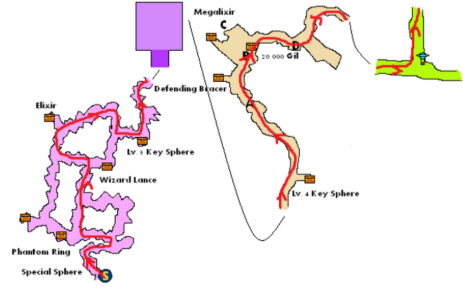
\includegraphics{graphics/sinpath}
	\item Before Seymour Omnis, \formation{\tidus}{\auron}{\yuna}
	\item Go up the steps, \sd
\end{enumerate}
\vfill
\begin{battle}[80000]{Seymour Omnis}
	\begin{itemize}
		\yunaf Defend
		\tidusf Armor Break
		\item \textit{If Armor Break Hit:}
		      \begin{itemize}
			      \auronf Defend
			      \summon{\bahamut}
			      \bahamutf Attack
		      \end{itemize}
		\item \textit{If Armor Break Missed:}
		      \begin{itemize}
			      \switch{\auron}{\rikku}
			      \rikkuf \od\ Mix Spherimorph Throwable + HiPot/MegaPot/XPot/Mega Phoenix
			      \yunaf Cure Mortiphasm
			      \tidusf Armor Break
			      \summon{\bahamut}
			      \bahamutf Attack
		      \end{itemize}
	\end{itemize}
\end{battle}
\begin{enumerate}[resume]
	\item \sd, walk north.
	\item \formation{\tidus}{\kimahri}{\auron}
	\item Make sure that \rikku's \od\ is charged. Can skip if using Skill Sphere for Armor Break.
	\item Turn left onto the bridge, go onto the next screen. \save\ if needed.
	\item Complete the minigame, picking up the eggs and avoiding the crystals.
\end{enumerate}
\end{multicols}
\begin{spheregrid}
	\begin{multicols}{2}
		\begin{itemize}
			\item \textit{If you got 2 or 4 \textbf{Return Spheres}:}
			      \begin{itemize}
				      \yunaf Attribute Sphere \rikku's +3 Agi (hold L)
				      \item Return Sphere ($\downarrow \downarrow \leftarrow \leftarrow$) or Friend Sphere ($\downarrow \leftarrow$) there
				      \item Go down, picking up Agi+4, Spare Change, Agi+4
			      \end{itemize}
			      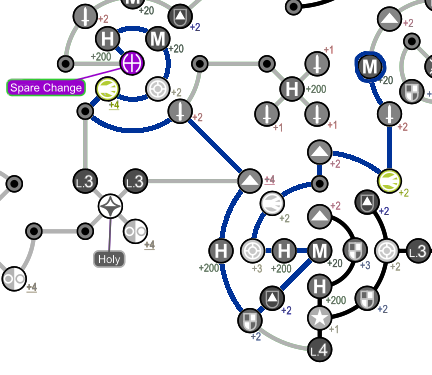
\includegraphics[width=.8\columnwidth]{graphics/4_Return_final_grid}
			\item \textit{If you got 0 \textbf{Return Spheres}:}
			      \begin{itemize}
				      \item Spare Change
				      \item Move $\swarrow$
				      \item Agi+4
				      \item Attribute Sphere Agi+3 at the start of \rikku\'s grid
				      \item Move to Mug $\searrow\rightarrow x7$
				      \item Agi+4
				      \item Move $\downarrow$
				      \item Agi+4
			      \end{itemize}
			      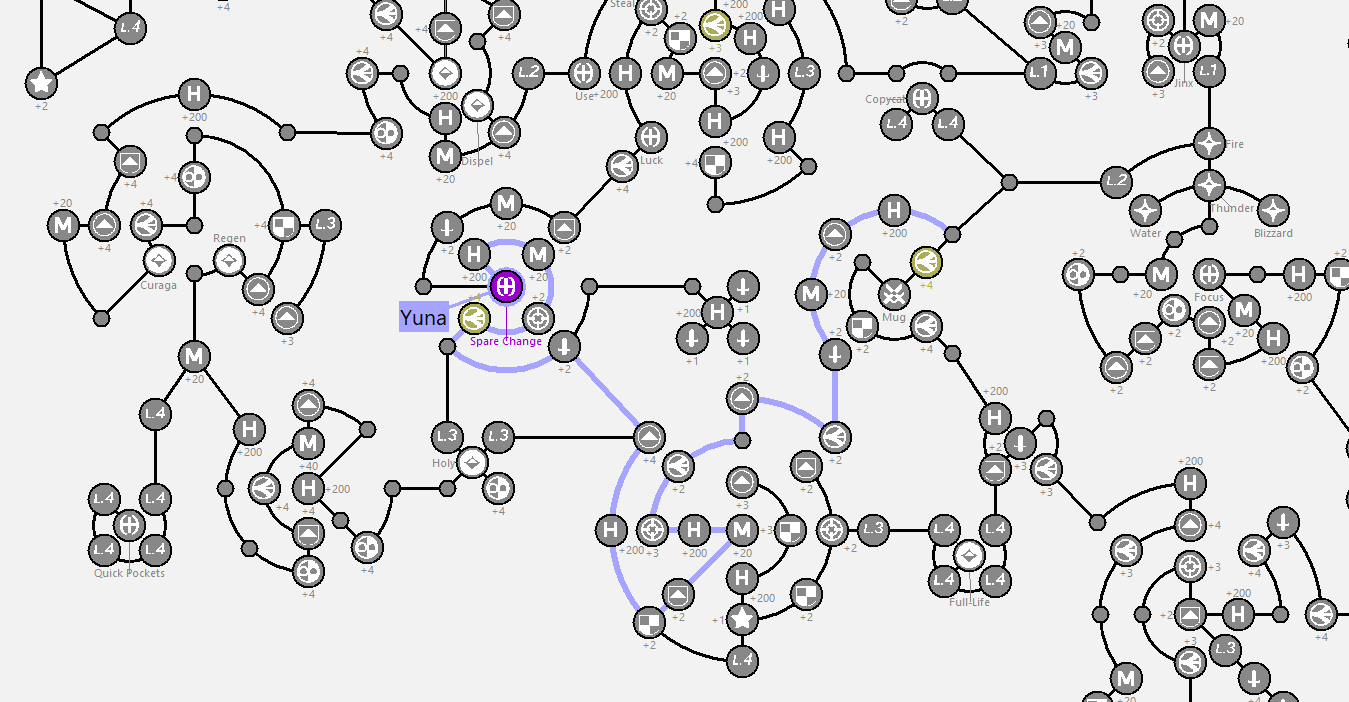
\includegraphics[width=.8\columnwidth]{graphics/0_return_before_BFA}
			      \columnbreak
			      \tidusf \textit{If you didn't get a \textbf{Zombie Strike} weapon}:
			      \begin{itemize}
				      \item \textit{If you got 2 or 4 \textbf{Return Spheres}:}
				            \begin{itemize}
					            \item Return $\uparrow\leftarrow$
					            \item Move $\uparrow$
					            \item Level 4 Keysphere
					            \item Move $\uparrow$
					            \item Zombie Attack
				            \end{itemize}
				      \item \textit{If you got 0 \textbf{Return Spheres}:}
				            \begin{itemize}
					            \item Move $\uparrow x5$
					            \item Level 4 Keysphere
					            \item Move $\uparrow$
					            \item Zombie Attack
				            \end{itemize}
						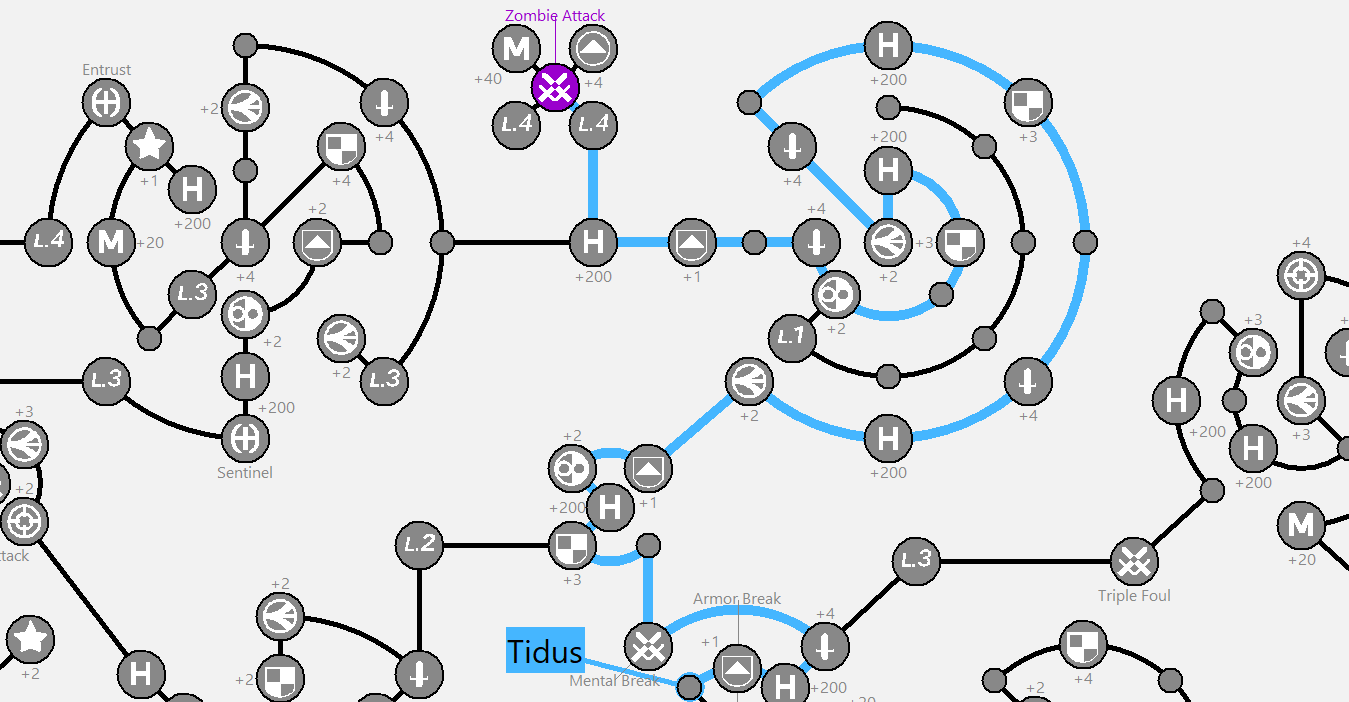
\includegraphics[width=.8\columnwidth]{graphics/Tidus_BFA}
			      \end{itemize}
				            \rikkuf If no \od, use Skill Sphere to learn Armor Break
		\end{itemize}
	\end{multicols}
\end{spheregrid}
\begin{multicols}{2}
	\begin{equip}
		\begin{itemize}
			\item Anyone that isn't \tidus, \yuna, \auron:
			      \begin{itemize}
				      \item Equip Zombie Strike Weapon
			      \end{itemize}
		\end{itemize}
	\end{equip}
	\begin{enumerate}[resume]
		\item Walk up to Jecht, \cs[4:30]
	\end{enumerate}
	\vfill
	\begin{battle}[180000]{Braska's Final Aeon}
		\begin{itemize}
			\switch{\yuna}{\rikku}
			\rikkuf \od\ Mix Grenade + HP Sphere or Armor Break
			\tidusf Talk
			\switch{\auron}{\yuna}
			\summon{\bahamut}
			\bahamutf Attack
		\end{itemize}
	\end{battle}
\end{multicols}
\begin{enumerate}[resume]
	\item \cs+\skippablefmv[4:00]
\end{enumerate}
\begin{battle}{Possesed Aeons}
	\begin{itemize}
		\item Spare Change as follows:
		      \begin{itemize}
			      \valeforf \num{20000} Gil
			      \ifritf \num{30000} Gil
			      \ixilonf \num{30000} Gil
			      \bahamutf \num{40000} Gil
			      \shivaf All Remaining Gil
		      \end{itemize}
	\end{itemize}
\end{battle}
\begin{enumerate}[resume]
	\item \cs[1:40]
\end{enumerate}
\begin{battle}[99999]{Yu Yevon}
	\begin{itemize}
		\item Zombie Attack:
		      \begin{itemize}
			      \yunaf Defend
			      \tidusf Zombie Attack
		      \end{itemize}
		\item \yuna\ Zombie Strike Weapon:
			\begin{itemize}
				\yunaf Switch Weapon
				\tidusf Switch Weapon
				\yunaf Attack
				\tidusf Phoenix Down Yu Yevon
			\end{itemize}
		\item \tidus\ Zombie Strike Weapon:
		      \begin{itemize}
			      \yunaf Defend
			      \tidusf Change Weapon
			      \tidusf Attack
		      \end{itemize}
		\item \rikku\ Zombie Strike Weapon:
		      \begin{itemize}
			      \yunaf Defend
			      \tidusf Haste \rikku
			      \yunaf Change Weapon
			      \rikkuf Attack
		      \end{itemize}
		\item \auron\ Zombie Strike Weapon:
			\begin{itemize}
				\switch{\yuna}{\auron}
				\auronf Change Weapon
				\tidusf Defend
				\auronf Attack
			\end{itemize}
		\item Anyone Else Zombie Strike Weapon:
		      \begin{itemize}
			      \switch{\yuna}{character with Zombie Strike Weapon}
			      \item That Character: Attack
			            \tidusf Phoenix Down Yu Yevon
		      \end{itemize}

		      \item Anyone: Phoenix Down Yu Yevon
	\end{itemize}
\end{battle}
\bothvfill
\begin{multicols}{2}